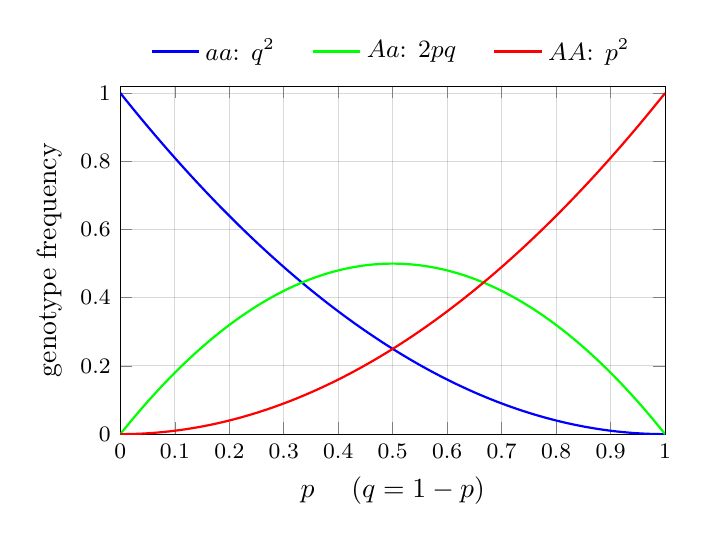
\begin{tikzpicture}
  \begin{axis}[
      width=8.5cm, height=6cm,
      xmin=0, xmax=1, ymin=0, ymax=1.02,
      xlabel={$p$ \quad ($q = 1-p$)},
      ylabel={genotype frequency},
      xtick={0,0.1,...,1}, ytick={0,0.2,...,1},
      grid=major, grid style={gray, opacity=0.3},
      legend style={at={(0.5,1.03)}, anchor=south, draw=none, legend columns=3, font=\small, /tikz/every even column/.append style={column sep=0.4cm}},
      tick label style={font=\footnotesize},
    ]
    \addplot[blue, thick, domain=0:1, samples=101] {(1-x)^2};
    \addlegendentry{$aa$: $q^2$}
    \addplot[green, thick, domain=0:1, samples=101] {2*x*(1-x)};
    \addlegendentry{$Aa$: $2pq$}
    \addplot[red, thick, domain=0:1, samples=101] {x^2};
    \addlegendentry{$AA$: $p^2$}
  \end{axis}
\end{tikzpicture}
